\section{The Out of Sample Error Rate}
%
%
\begin{frame}
  The goal in building a predictive model is often to find an
  appropriate functional form that minimizes the expected error
  rate:
  $$\ESE(f) = E \left[ \left( y - f(x) \right)^2 \right]$$
\end{frame}
%
%
\begin{frame}
  In this section, we turn our attention to estimating this quantity.
\end{frame}
%
%
\begin{frame}
  The first difficulty is that there are different ways to interpret the error,
  depending on what is or is not considered at random.
\end{frame}
%
%
\begin{frame}
  We have already discussed the error when randomizing over both a training set
  and an out of training sample, called the \textbf{expected out of sample
  error}:

  $$\ESE = E_{X,Y,\D} \left[ \left( y - f(x; \D) \right)^2 \right]$$

  It is this quantity that we were able to decompose with the
  \textbf{bias-varaince} decomposition.
\end{frame}
%
%
\begin{frame}
  Possibly more relevant, is the error when randomizing over an out of training
  sample, but for a \textit{fixed} training set:

  $$\ESE(\T) = E_{X,Y} \left[ \left( y - f(x; \T) \right)^2 \right]$$
\end{frame}
%
%
\begin{frame}
  Also convenient is the \textbf{expected training error}, where the sample error is
  computed on the same dataset used to train the model:

  $$\ETE = E_{\T} \left[ \frac{1}{N} \sum_{x,y \in \T} (y - f(x; \T))^2 \right] $$
\end{frame}
%
%
\begin{frame}
  The expected training error is \textit{not} a good estimator of the expected
  out of sample error, because the modeling algorithm incentives fitting the
  training data as closely as possible:
  \begin{figure}
    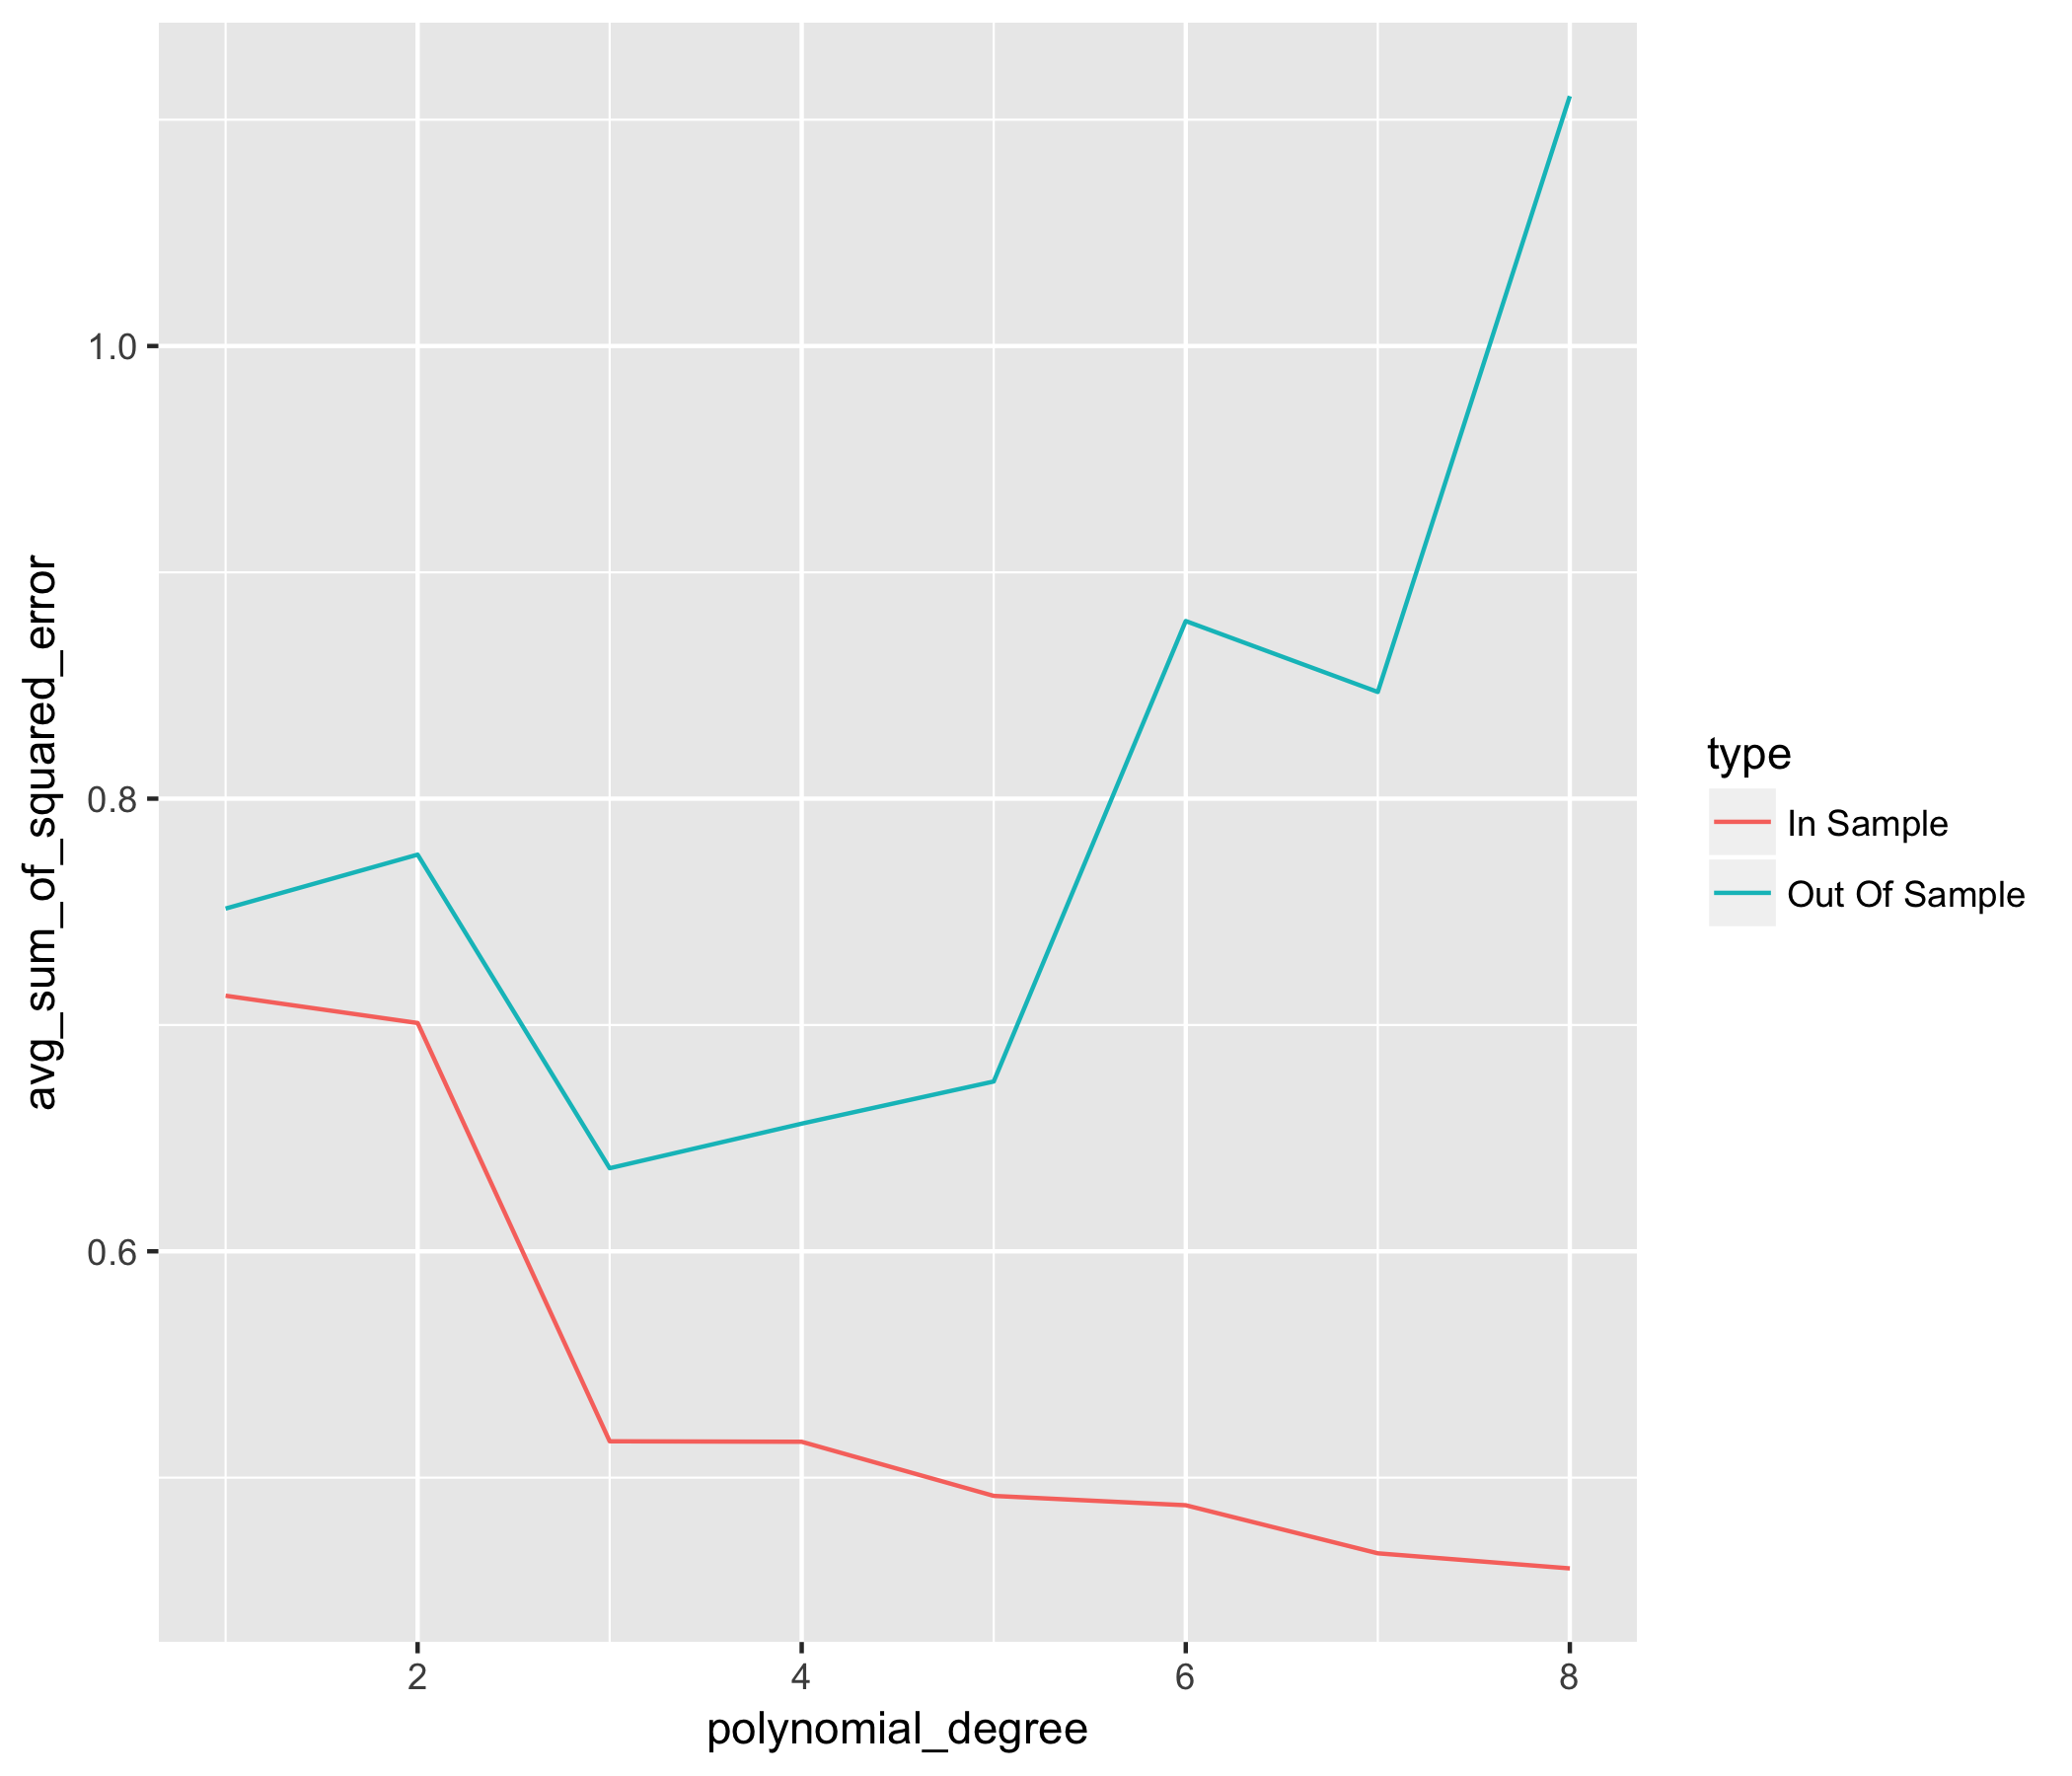
\includegraphics[scale=0.09]{learning_curves_by_degree}
  \end{figure}
\end{frame}
%
%
\begin{frame}
  The effect is amplified in high model variance situations (small data sets or
  noisy data):
  \begin{figure}
    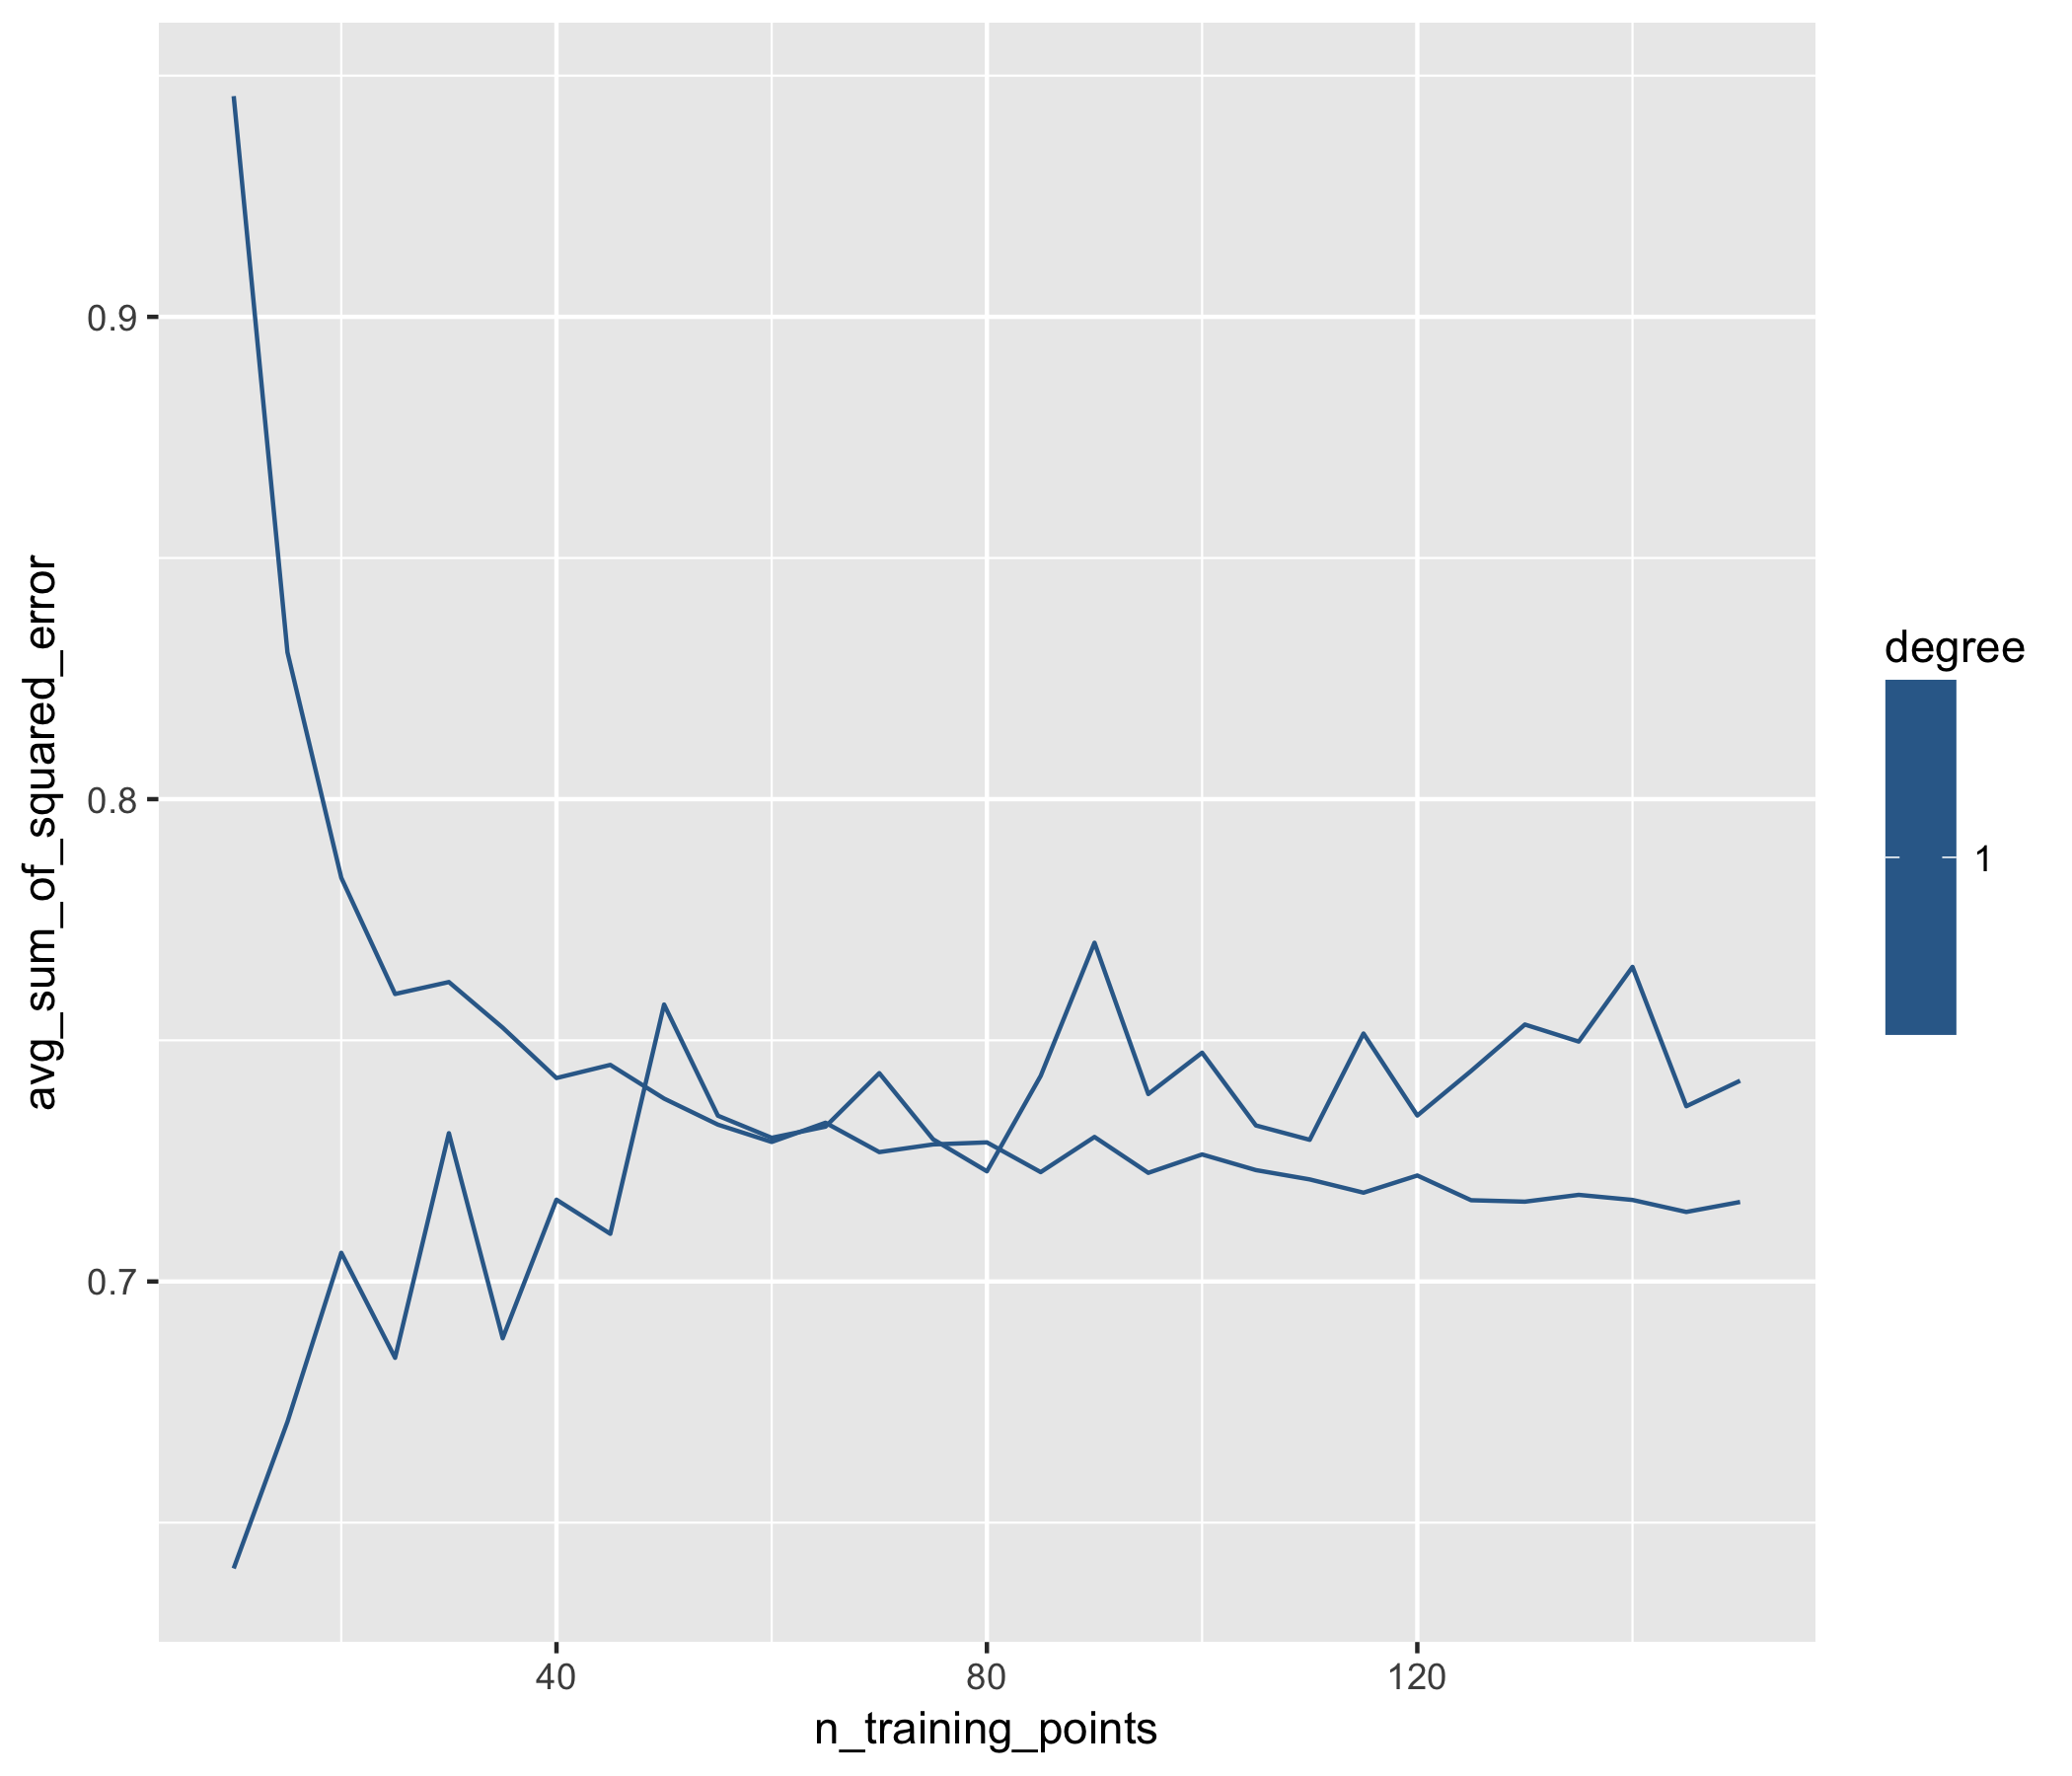
\includegraphics[scale=0.09]{in_and_out_of_sample_learning_curves}
  \end{figure}
\end{frame}
%
%
\begin{frame}
  The bias of the in sample error is so important, it's worth putting some math behind it:
  \begin{align*}
    \ESE &= E_{X,Y,\T} \left[ \left( y - f(x; \T) \right)^2 \right] \\
         \only<2->{
           &= E_{\D, \T} \left[ \frac{1}{N} \sum_{x,y \in \D} (y - f(x; \T))^2
           \right] \\
         }
         \only<3>{
           &\geq E_{\D} \left[ \frac{1}{N} \sum_{x,y \in \D} (y - f(x; \D))^2 \right]
         }
         \only<4>{
           &\geq E_{\T} \left[ \frac{1}{N} \sum_{x,y \in \T} (y - f(x; \T))^2 \right]
         }
  \end{align*}

  \only<2>{
    We can replace the expectation of distribution with the expectation of its
    sample means.
  }
  \only<3>{
    This is the definition of $f(X, \D)$, it has smaller error than all other
    possible $f$ when the sample error is evaluated on $\D$.
  }
  \only<4>{
    Changing the name of a free variable.
  } 
\end{frame}
%
%
\begin{frame}
  Since the training error is not a good estimate of the out of sample error, we
  need an alternative way to get at this quantity.  There are two major
  approaches:
  \begin{itemize}
    \item Using a \textbf{hold out set}.
    \item Using \textbf{cross validation}.
  \end{itemize}
\end{frame}
%
%
\begin{frame}
  If a dataset $\Holdout$ has participated in neither the training of the model, or
  the decision making process, then:

  $$ \frac{1}{N} \sum_{x,y \in \Holdout} (y - f(x; \T))^2 $$

  is an unbias estimate of $\ESE(\T)$ (the expected out of sample error with a
  fixed training set).
\end{frame}
%
%
\begin{frame}
  Holding out data is \textit{not} costless, as there is less data available for
  training and a smaller data set will increase the variance of the estimated
  model:
  \begin{figure}
    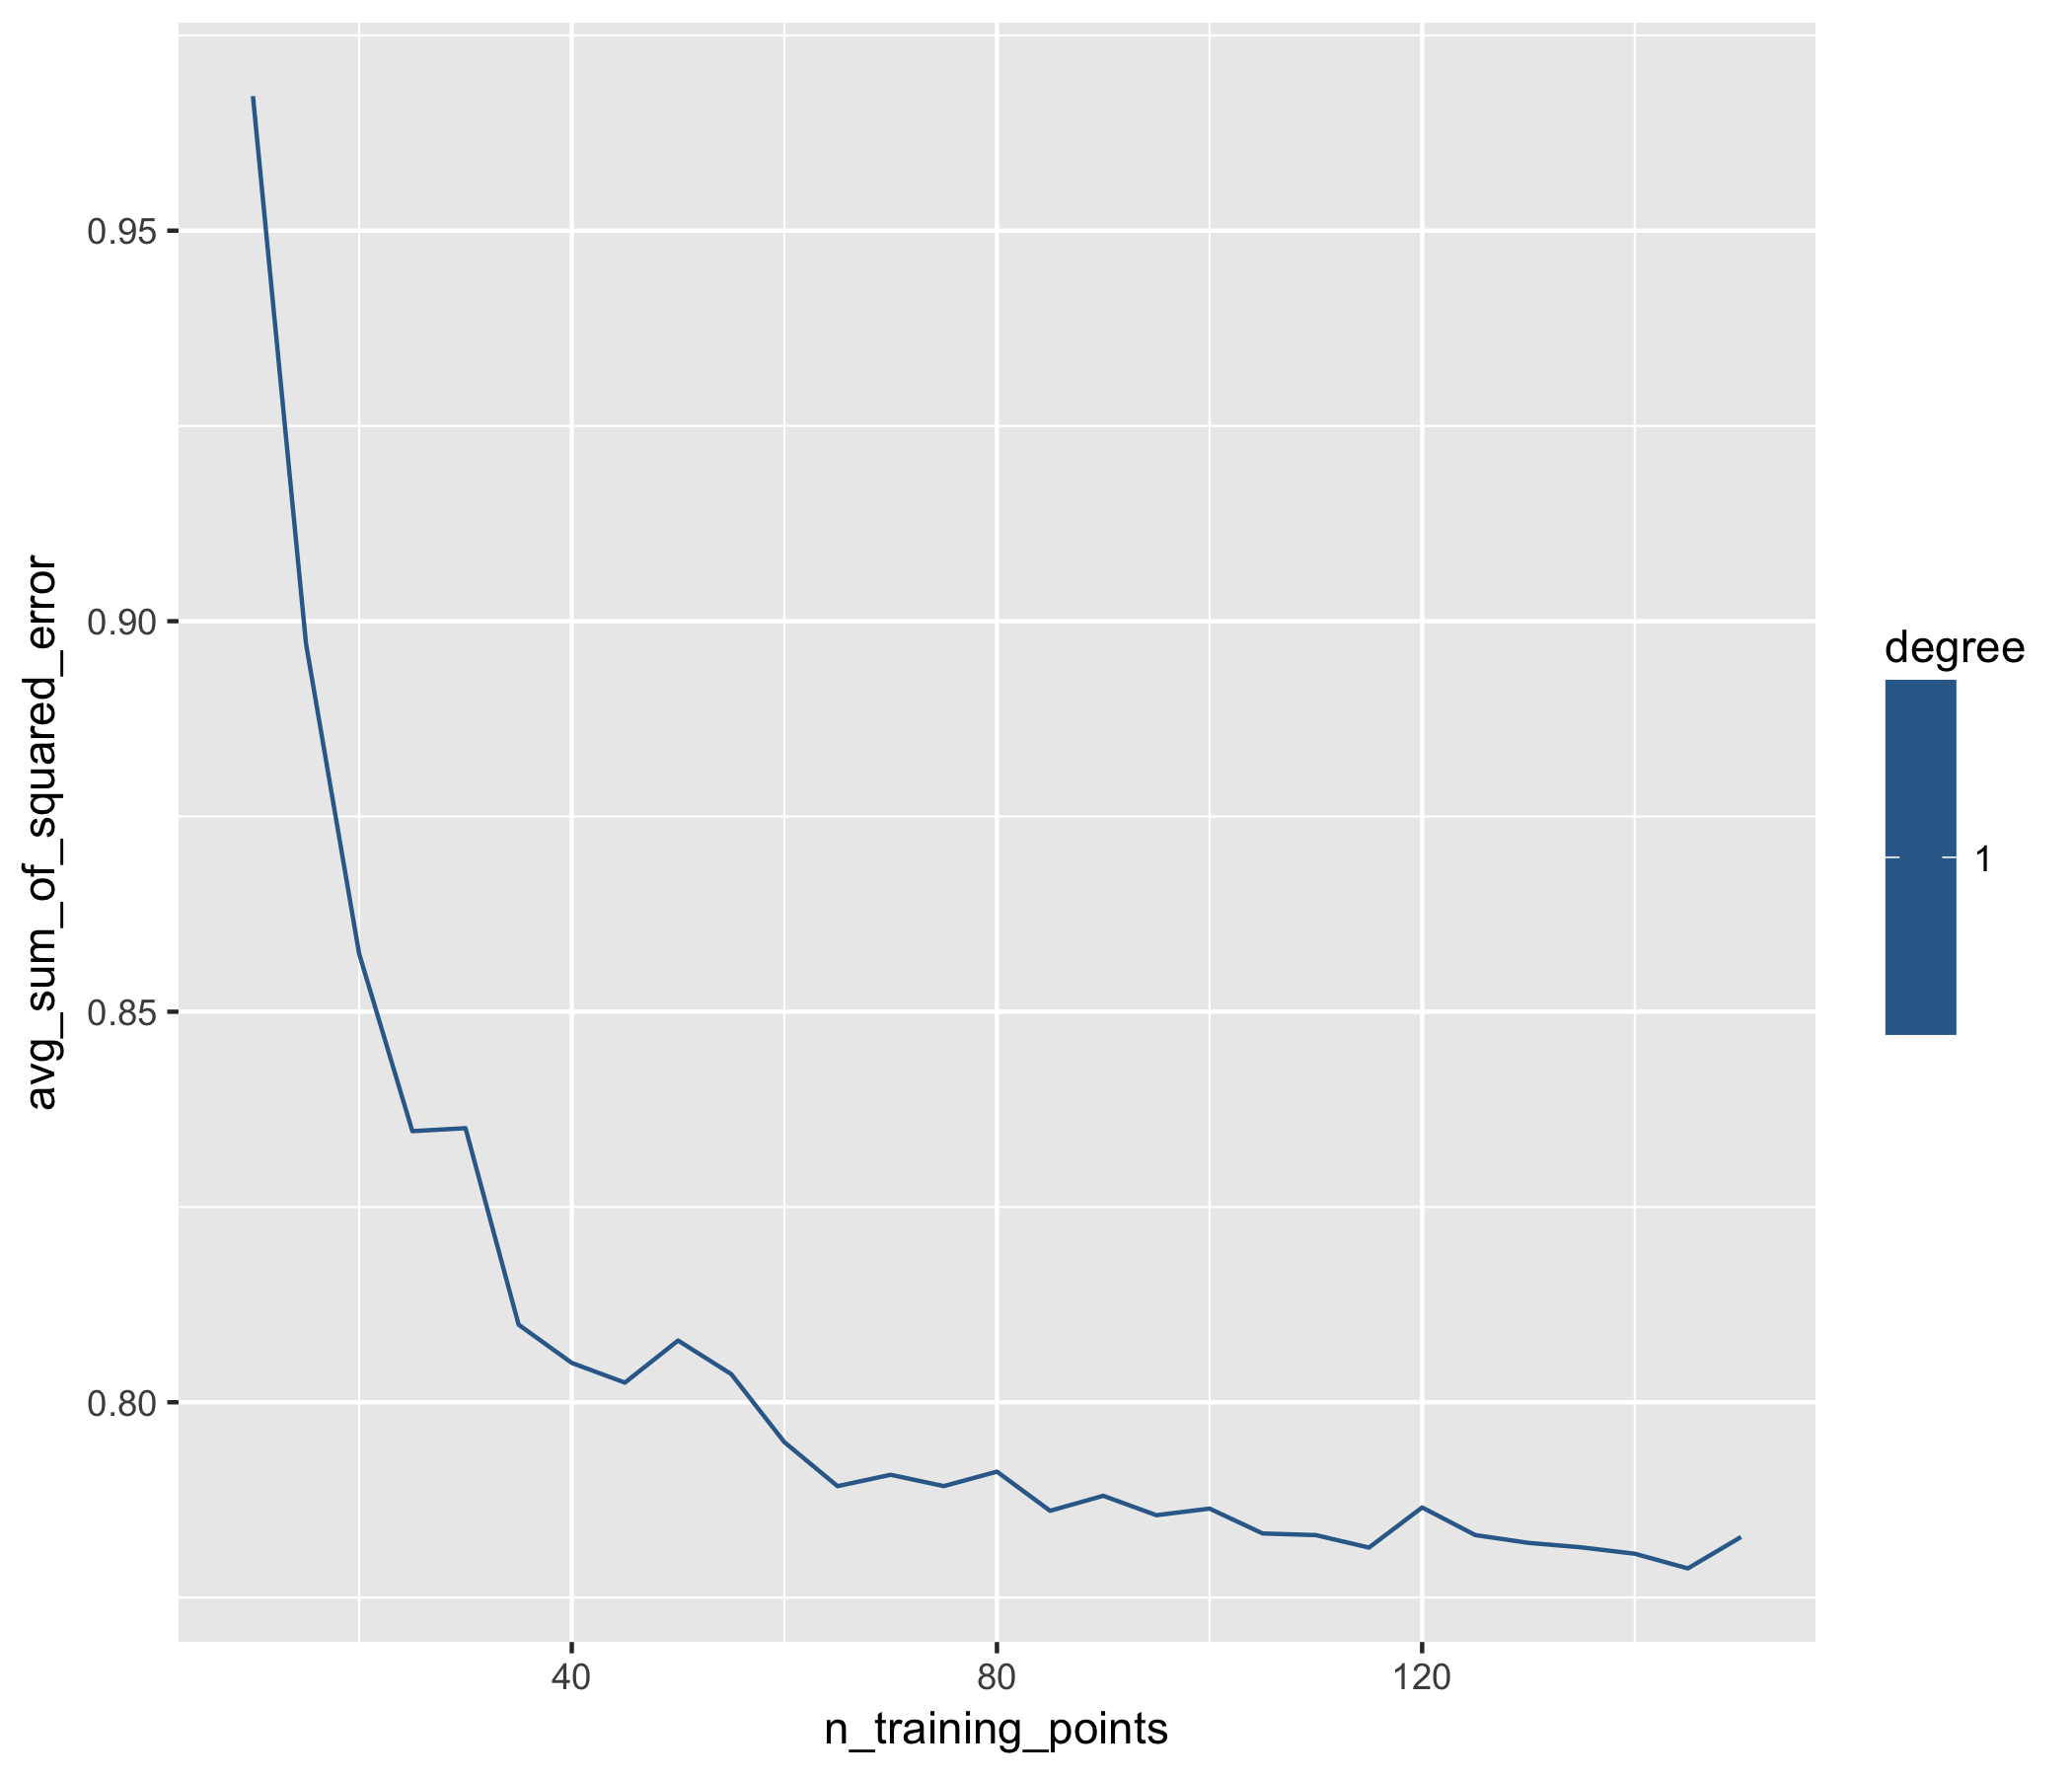
\includegraphics[scale=0.08]{out_of_sample_learning_curve}
  \end{figure}
  How costly holding out data is depends on the shape of the learning curve for
  the model being estimated.
\end{frame}
%
%
\begin{frame}
  \begin{figure}
    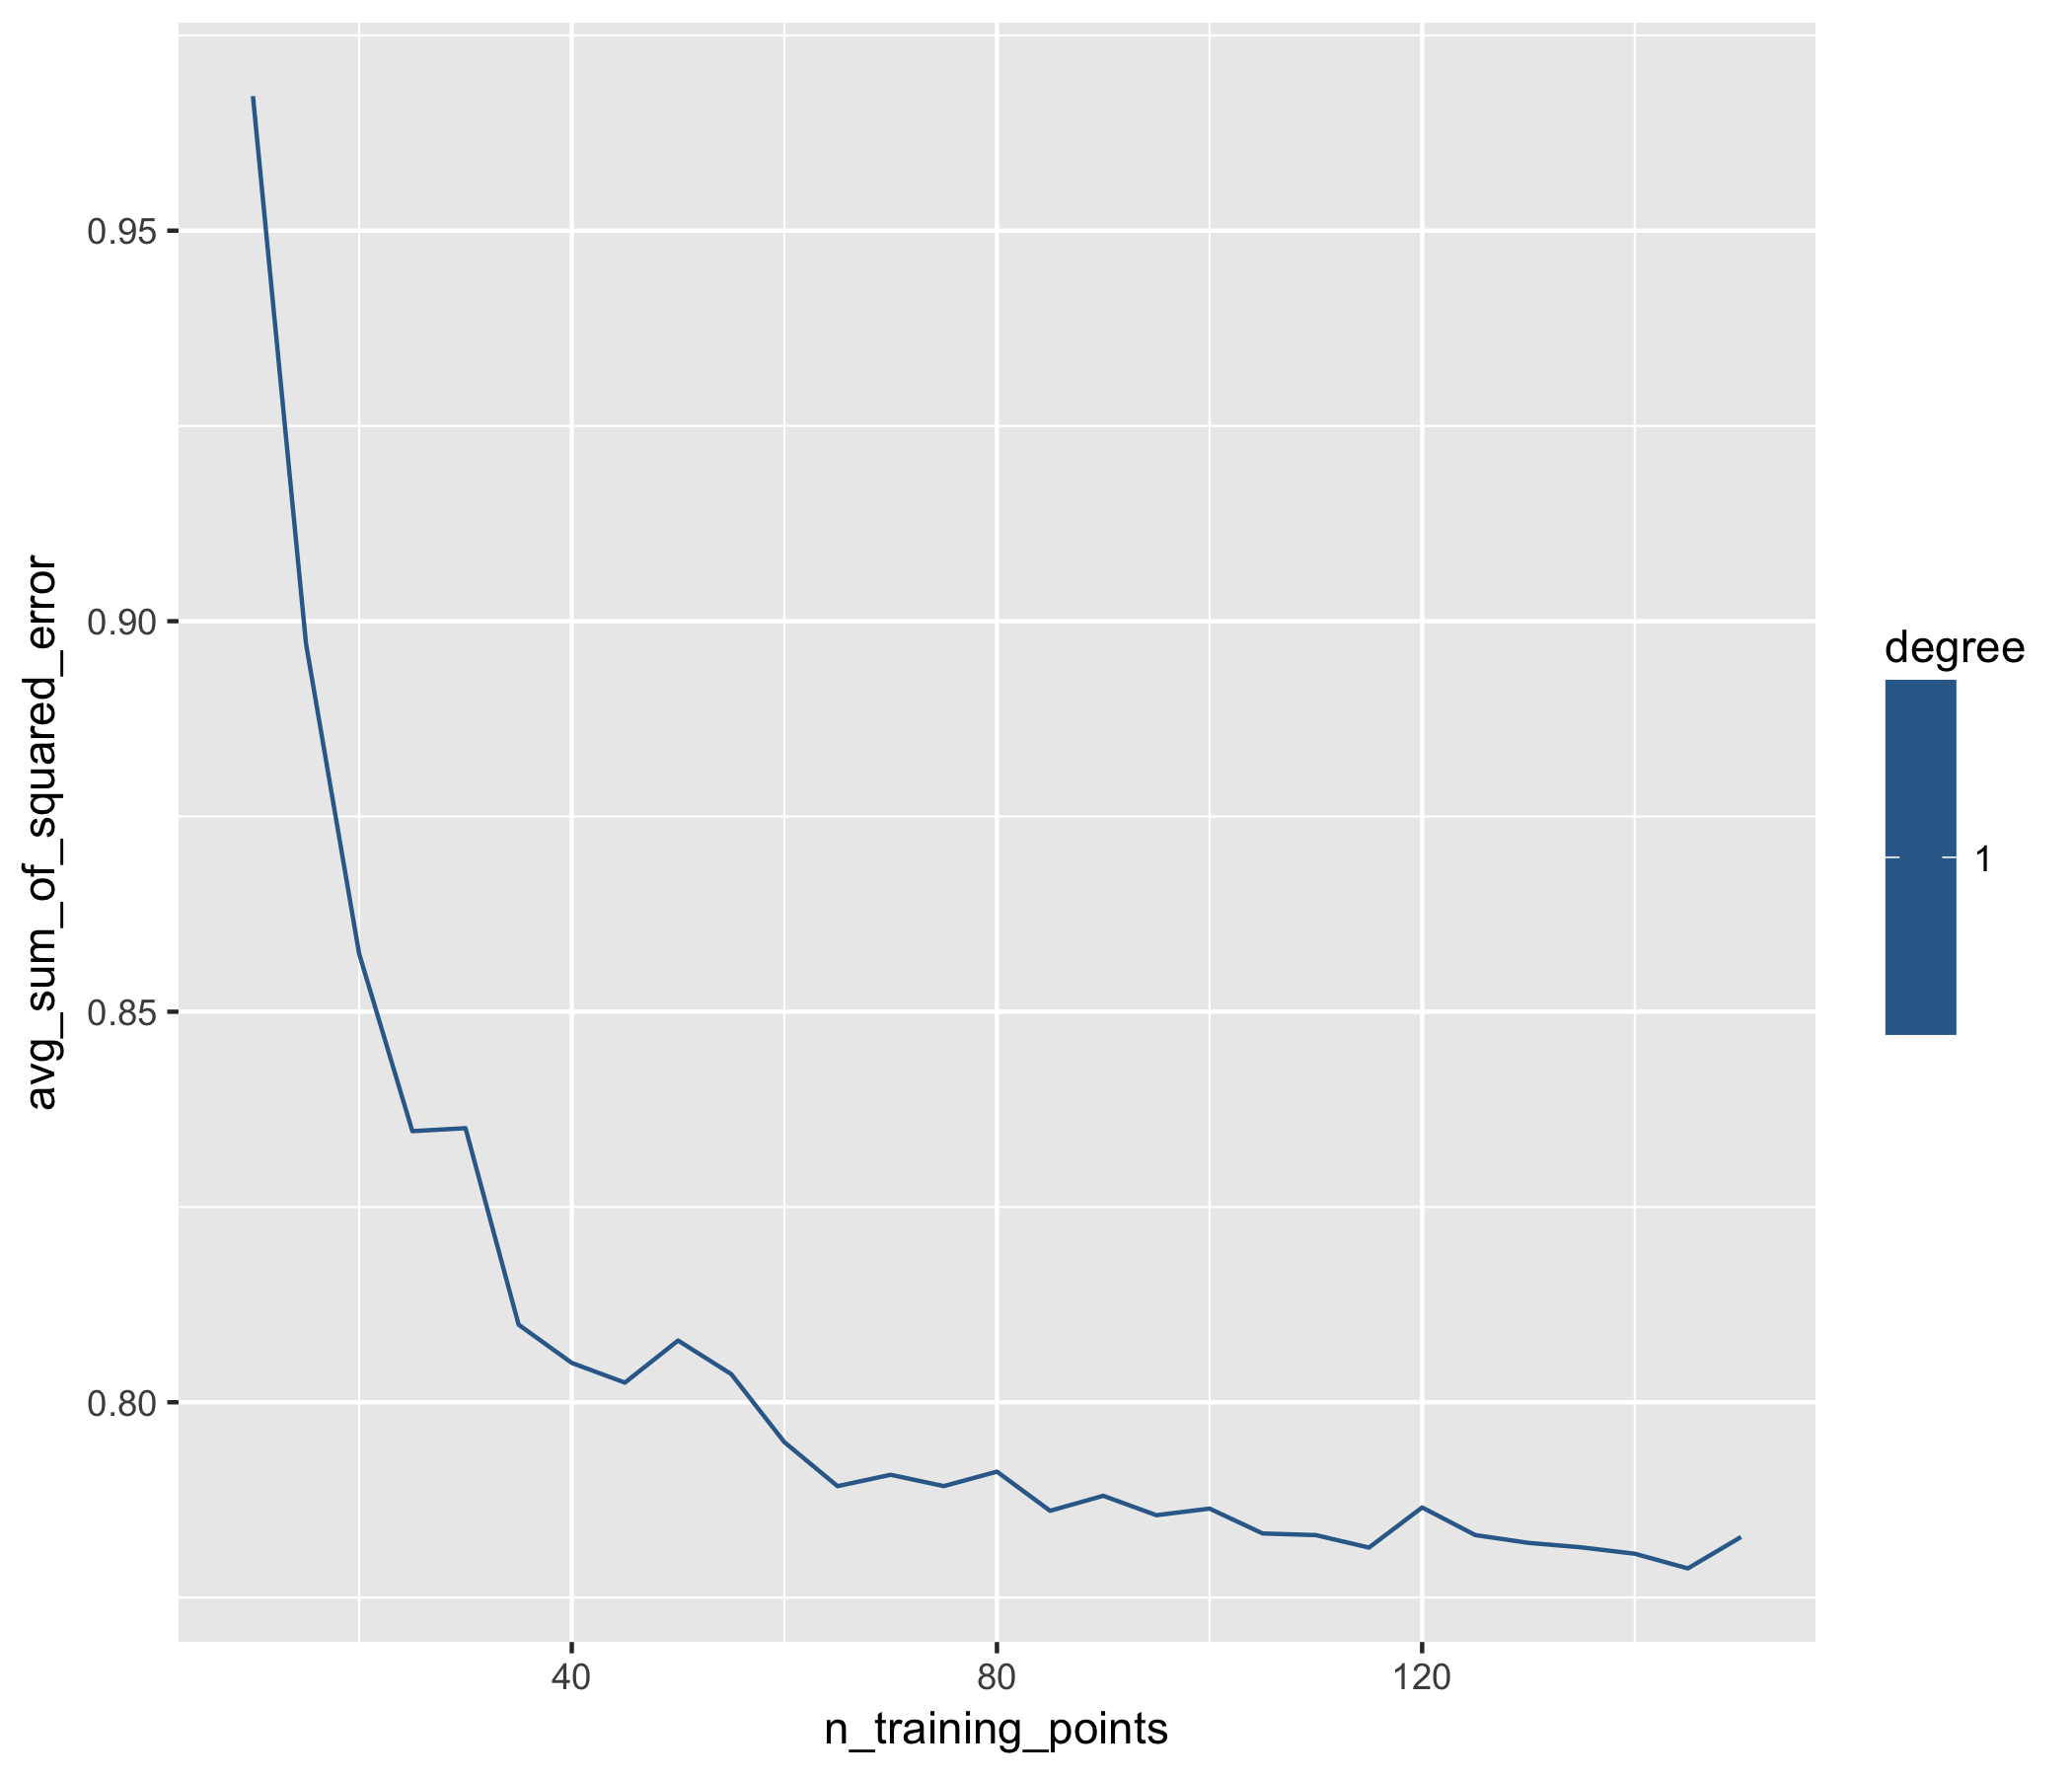
\includegraphics[scale=0.08]{out_of_sample_learning_curve}
  \end{figure}
  This shape is affected by:
  \begin{itemize}
    \item The overall level of noise in the data (irreducible error).
    \item The complexity of the model being estimated.
  \end{itemize}
  Noisier data and more complex models may be more adversely affected by holding
  out data.
\end{frame}
%
%
\begin{frame}
  In \textbf{cross validation} the data is available is partitioned into a
  disjoint union of \textit{folds}:
  $$ {\T} = {\T}_1 \cup {\T}_2 \cup \cdots \cup {\T}_k $$
  For each $i$, the out of fold data is formed by removing the fold ${\T}_i$ from
  the training data set:
  $$ \hat{{\T}}_i = {\T}_1 \cup \cdots \cup {\T}_{i-1} \cup {\T}_{i+1}
  \cup \cdots \cup {\T}_k $$
\end{frame}
%
%
\begin{frame}
  The cross validation estimate of the out of sample error is:
   $$ \frac{1}{k} \sum_{i=1}^{k} \frac{1}{\# {\T}_i } \sum_{x,y \in
   {\T}_i} (y - f(x, \hat{{\T}}_i))^2$$ 
   Since we are randomizing over a training set, this is actually an estimate of
   $\ESE$.
\end{frame}
%
%
\begin{frame}
  That is, while the hold out sample error is an estimate of:
  $$\ESE(\T) = E_{X,Y} \left[ \left( y - f(x; \T) \right)^2 \right]$$
  The cross validation estimate is of:
  $$\ESE = E_{X,Y,\D} \left[ \left( y - f(x; D) \right)^2 \right]$$
\end{frame}
%
%
\begin{frame}
  The number of folds to use is yet another example of balance and compromise in
  statistical modeling.
\end{frame}
%
%
\begin{frame}
  If a small $k$ is chosen, much data is held out from each training set,
  depending on how much total data is available, this can increase the variance
  of the estimated model:
  \begin{figure}
    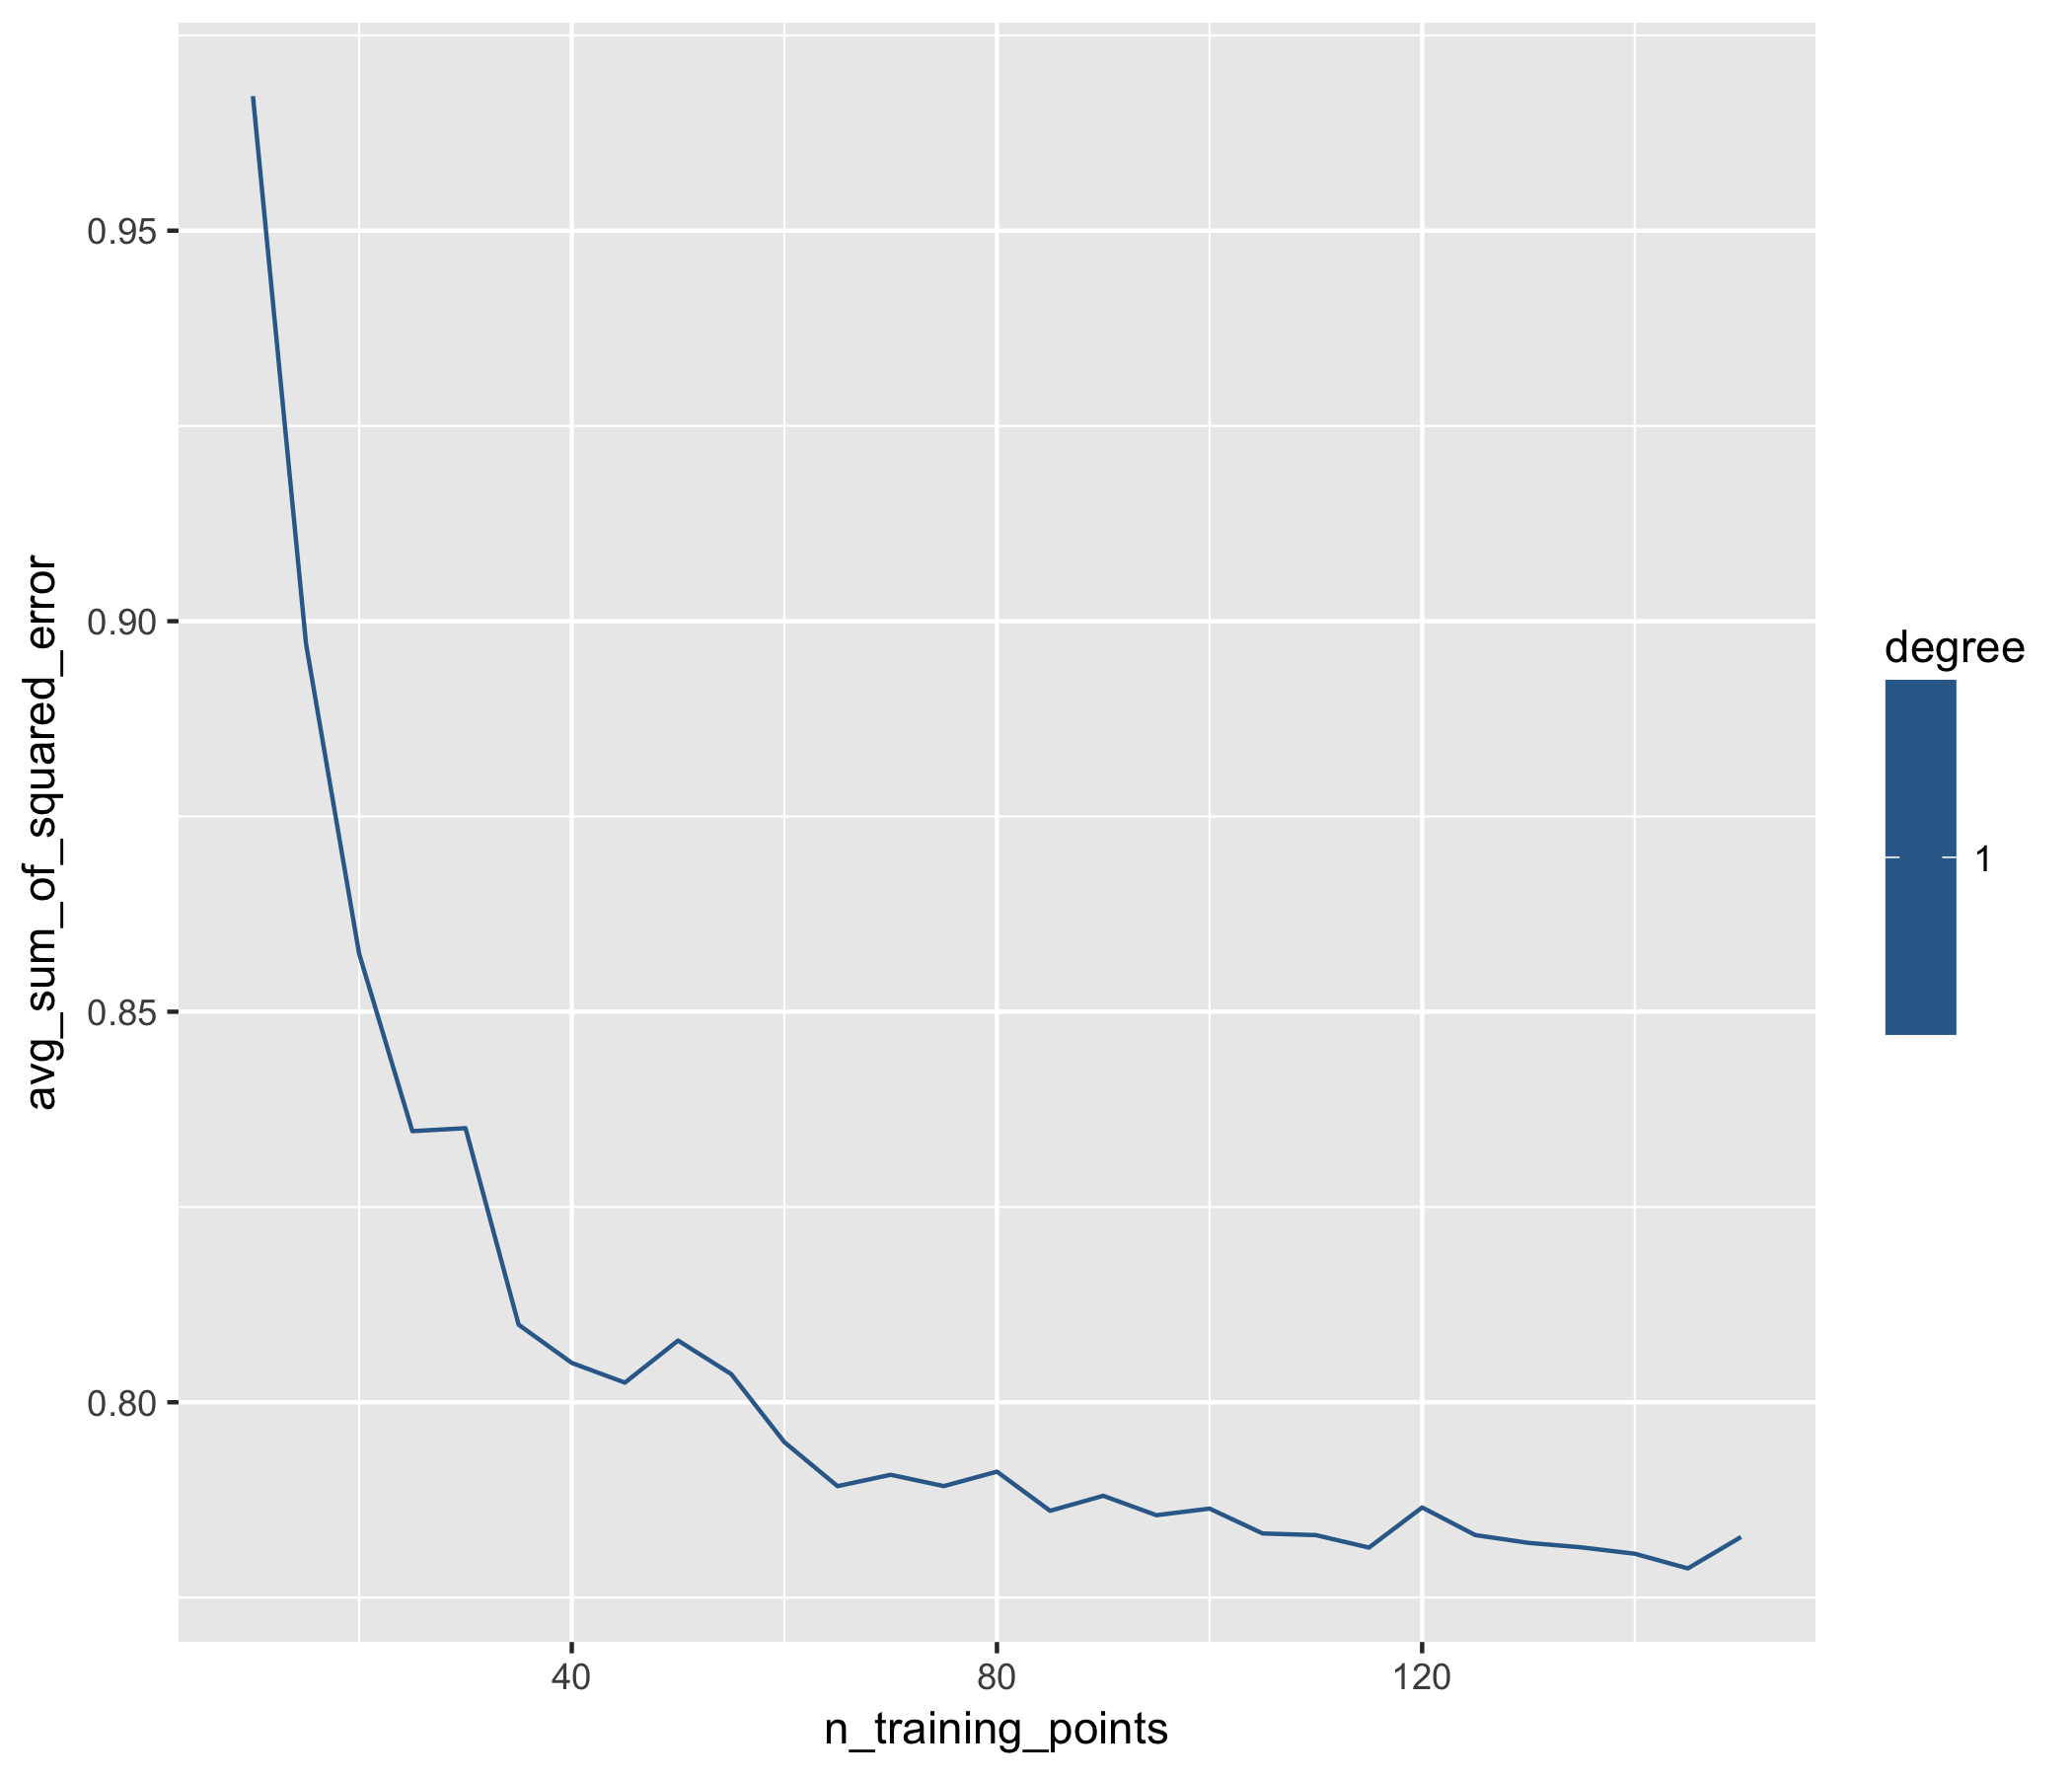
\includegraphics[scale=0.09]{out_of_sample_learning_curve}
  \end{figure}
\end{frame}
%
%
\begin{frame}
  At the other extreme, the $k = N$ case is called \textbf{leave one out cross
  validation}.  In this case the models trained on the complementary sets are
  highly correlated, as the various training sets differ at only one point:

  $$ f(x, \hat{{\T}}_i) \approx  f(x, \hat{{\T}}_j) $$
\end{frame}
%
%
\begin{frame}
  This makes the cross validation estimator relatively insensitive to model
  variance, as the training data is not sufficiently averaged out.

  Said another way, if the cross validation estimate is repeated over various
  \textit{full} training sets, \textit{this estimate} will have high variance.
\end{frame}
